%------------------------------------------------------------------------------------------------------------------------------------------
%  Teorie
%------------------------------------------------------------------------------------------------------------------------------------------
\chapter{TEORETICKÁ VÝCHODISKA}
\par Pro plné pochopení, výběru a případném vypracování platformz je potřeba si objasnit a vysvětlit několik témat. Jsou to především \textit{Vývojové platformy low-code}, výsledná platforma by měla splňovat tuto definici. Dále si objasníme pojemy \textit{Bussiness intelligence} (platforma bude z části pracovat s touto oblastí) a \textit{Platforma pro pokročilou vizualizaci dat} -- pro snadné používání uživatelského rozhraní. A vzhledem k tomu že výsledná platforma musí do určité části pracovat s uživatelskými právy a spravovat uživatele, objasníme si pojem \textit{Server pro řízení přístupu a identity}

\section{Vývojové platformy low-code}
\par Vývojové platformy low-code jsou celkem nový pojem, tyto produkty začali vznikat, protože malé a střední podniky potřebovali vytvořit rychle a za použití menšího počtu vývojářů aplikace, které mohou být nadále rychle spravovány. \cite{pcmag-no-coding}

\par Toto v podstatě znamená, že vývojáři mohou rychle měnit software na základě uživatelských požadavků, což má za následek spokojenější uživatele, uživatelsky přívětivější software a toto všechno za minimálního použití ručního programování. Takovéto platformy neeliminují programování jako takové, ale napomáhají rychlejšímu vývoji, tak že poskytují vizuální nástroje a napomáhají konfiguraci datových modulů a pomáhají eliminovat problémy spojené s  datovou integrací. \cite{low-code-customer-want}

\subsubsection{Výhody low-code platforem}
\begin{itemize}
  \item \textbf{Produktivita:} Systémy mohou být vyvýjeny a nasazeny během menšího časového rozmezí, oproti klasickému programování. \cite{low-code-accelerate}
  \item \textbf{Reakční schopnost:} Vývojář může často zvolit různé druhy platforem na kterých bude výsledný produkt fungvat, od mobilních aplikací, až po webové služby. \cite{low-code-accelerate}
  \item \textbf{Spolehlivost:} Aplikace mohou být aktualizovány mnohem rychleji, což má za následek jejich stabilitu a spolehlivost. \cite{low-code-accelerate}
  \item \textbf{Úspora času a peněz:} Vývojáři mohou vytvořit mnohem více funkcionality za kratší čas, z čehož plyne že si firma může dovolit mensí počet programátorů. \cite{low-code-accelerate}
  \item \textbf{Zaměření na samotný vývoj:} Zaměřením na to co má aplikace dělat, a ne jak to má dělat, programátoři se mohou zaměřit na funkcionalitu a uživatelskou spokojenost. Při vývoji je možné se zaměřit také více na uživatelské požadavky mnohem rychleji. \cite{low-code-accelerate}
\end{itemize}

\subsection{Příklady low-code platforem}
\paragraph{Microsoft PowerApps} Vývojová platforma od firmy Microsoft, která dovoluje vytvořit během několika málo kliknutí aplikaci pro mobilní platformy a také jako webové služby. Při spojením této platformy a aplikace Power BI vzniká velice robustní vývojářský nástroj, díky kterému je možné rychle integrovat produkční data do aplikace, kterou budou uživatelé rádi používat. \cite{pcmag-no-coding}
\paragraph{Zoho Creator} Výhodou této platformy je využití techniky \uv{\tt{drag-and-drop}}, která umožňuje vytvářet aplikace a převážně jejich uživatelské rozhraní bez nutnosti psát jakýkoliv kód. \cite{zoho-review}
\paragraph{Rollbase} Při používání této platformy vývojář jako první definuje objekty, jejich vlastnosti a vztahy mezi těmito objekty. Po překonání tohoto kroku máme již plně funkční webovou aplikaci, která je funkční napříč všemi mobilními zařízeními. \cite{what-is-low-code}
\paragraph{Openshift} Platforma pro vývoj webovým a mobilních aplikací, postavená na kontejnerech, které zajišťuí rychlý vývoj a možnost dedikovat vývojáře na vytvoření jednoduchých funcionalit jako samostatné aplikace \footnote{Takovýmto aplikacím se říka Microservice \url{https://smartbear.com/learn/api-design/what-are-microservices/}}, které za pomocí Openshiftu vytvoří velkou a komplexní aplikaci. Na Obrázku \ref{openshift-vrstvy} můžeme vidět z jakých vrstev se skládá Openshift a můžeme vidět jednotlivé aplikace zázorněné v nodech, dále můžeme vidět jaké nástroje nabízí Openshift vývojářům (management zdrojových kódů -- SCM a kontonualní integrace -- CI/CD).\cite{openshift-overview}
\begin{figure}[h]
\label{openshift-vrstvy}
\centering
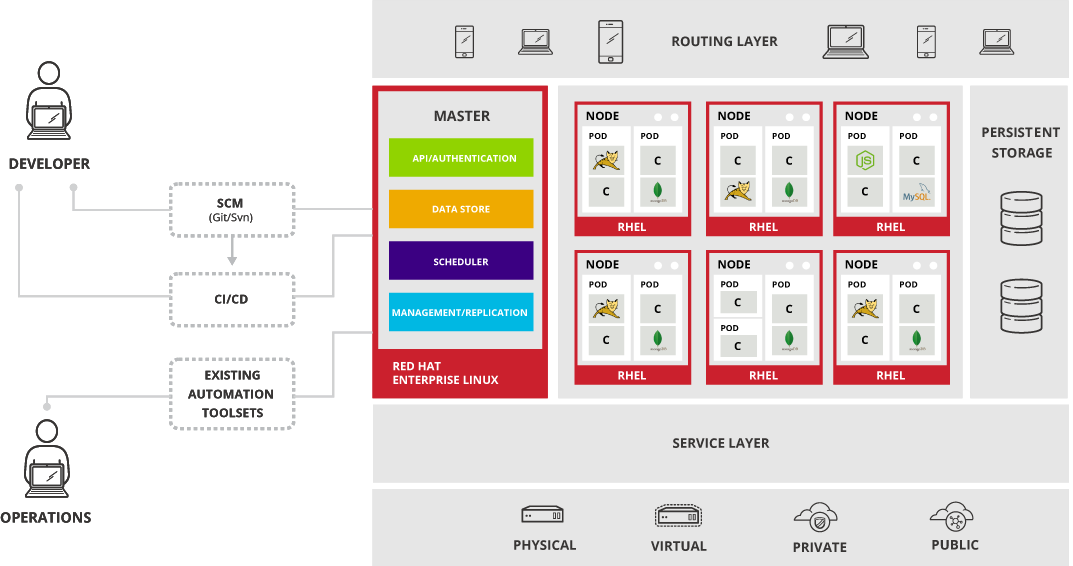
\includegraphics[width=\textwidth]{openshift}
\caption{Znozornění jednotlivých vrstev v platformě openshift.}
\end{figure}

\subsection{Cloudový výpočet}
\par Výpočet pomocí cloudu je další fáze ve vývoji internetu, cloud v tomto použití znamená že všechno potřebné pro vývoj a hostování aplikací, až po samostatné stroje je možné nabídnout jako služba kekoliv na světě se člověk nachází. I když poskytovatelé cloudových řešení mají často velice robustní bezpečnostní systém je na uživateli, který má uložené data v cloudu, aby zajistil jejich bezpečnost. To znamená že pokud data uniknou z cloudu díky špatnému zabezpečení v aplikaci, která je hostovaná, není chyba poskytovatele, ale firmy, která takovou aplikaci vydala.\cite{cloud-computing-dummies}

\par Pporovnání ceny cloudového výpočtu a klasického datavého uložiště není až tak jednoduché, záleží na někkolika faktorech. Vezměme si například lokaci datového uložiště, pokud například cena elektické energie v místě datového uložiště je velice levná firma nemusí být tolik tlačena do cloudového řešení. ale pokud k těmto datům přistupuje velké množství uživatelů z různých koutů světa může se stát že námi poskytované služby budou neresponzivní a uživatelé mohou odejít ke konkurenci. V tomto momentě je potřeba zvážit zda se nám cloudové řešení vyplatí a kdy ne. Důležité je také uvědomit si, že 42 \% nákladů na datové uložiště jde do hardware a software (tyto náklady jsou rozloženy v průběhu času) a 58 \% nákladů jde do topení, klimatizace, daní a samostatné práce. \cite{cloud-computing-dummies}

\subsubsection{Typy cloudového výpočtu}
\begin{itemize}
  \item \textbf{Veřejné} dostupné pro širokou veřejnost, jak zdarma, tak placené verze.
  \item \textbf{Soukromé} často používané firmami skupinami uživatelů, kteří potřebují zabezpečit data. Často velice drahé a ačasově nákladné řešení.
  \item \textbf{Komunitní} podobné soukromým, ale rozšířené mezi větší skupiny lidí.
  \item \textbf{Hybridní} vytvořené z jednoho a více druhů, privatního a nebo veřejného cloudu. Mezi jejich portfoliočastopatří zálohakekritickýmslužbám.
  \item \textbf{DaaS} data jako služba, pouze data uložené v cloudu.
  \item \textbf{PaaS} pro vývoj a hostování celého vývojového cyklu, často všetně možnosti nasazení výsledné aplikace.
  \item \textbf{IaaS} infrastruktura jako služba, opravdové, nebo virtuální počítače nabízené uživatelům. \cite{cloud-computing} \label{IaaS}
\end{itemize}

\subsubsection{Platforma jako služba -- PaaS}
Platforma jako služba tento pojem označuje službu, která zahrnuje kompletní škálu nástrojů sloužících pro vývoj aplikací. Od databází, přes aplikační rámce a testovací nástroje až po nasazení a překlad aplikace. Výhoda této služby je převážne v tom, že všechno je přístupné přes internet a často jako webová aplikace, takže není nutné kupovat často velice drahé nástroje. Někteří poskytovatelé nabízí také vyrovnání zatížení, to znamená že pokud je výsledná aplikace pod vysokým náporem uživatelů, automaticky se přiřadí prostředky, aby uživatelé nezaznamenali pád aplikace a bez nutnosti zasáhnout do nastavení služby.\cite{essentials-cloud}

\subsubsection{Výhody PaaS} 
\begin{itemize}
  \item \textbf{Méně kódu} -- Díky možnosti projení několika menších aplikací dohromady není potřeba psát stejný kus kódu pořád dokola.
  \item \textbf{Nové možnosti bez potřeby nabírání nových lidí} -- Díky PaaS dostane tým do rukou sofistikovanější nástroje.
  \item \textbf{Vývoj pro více platform} -- Výhodou mnoha poskytovalů služby PaaS je možnost překladu aplikací pro různé platformy (několik mobilních platforem a webová aplikace).
  \item \textbf{Propojení geograficky nesourodých týmů} -- Pokud je tým rozdělen po různých částech světa služby PaaS dovolují takto rozděleným týmům pracovat efektivněji.
  \item \textbf{Efektivní životní cyklus aplikace} -- V rámci integrovaného prostředí se často nachází funkce pro podporu životního cyklu aplikace (sestavení, nasazení, otestování, správa, aktualizace...). \cite{co-je-paas}
\end{itemize}

\section{Bussiness Intelligence}
\par Nástroje pro bussiness Intelligence zahrnují jak samostatná data, tak časovou jednotku, takže můžeme nad těmito daty provádět predikci pomocí sofistikovaných nástrojů a výpočtů. Ze začátku byo jednoduché provádět takové výpočty, protože jednoduše firma nesbírala takové množství dat. Aktuálně však není v lidských silách provádět takové výpočty nad tak obrovským množstvím dat. \cite{data-science-business}

\par Pravděpodobně nejvíce rozšířeným aplikováním data-miningu je marketing -- sledování nakupování a chování zákazníků. V této oblasti je možné vybrat si každého zákazníka, a v případě že máme dostatek dat, cílit na něj lépe reklamu. \cite{data-science-business}

\par Pro plné využití BI nástrojů potřebujeme sledované subjekty rozdělit do několika skupin, tyto skupiny musí být co nejvíce \textbf{Heterogenní} (rozdílné) vůči sobě, a subjekty v rámci jedné skupiny musí být na druhou stranu co nejvíc \textbf{Homogenní} (stejné). Pokud sledované subjekty spadají do více skupin (toto se může hodit z mnoha důvodů) můžeme použít takzvané  \textbf{Clustery}. Což jsou skupiny objektů, které si jsou co nejvíce podobné, ale objekty v jiné skupině se jim budou co nejvíce lišit. \cite{data-science-business}

\par Samostatá data jako taková však nejsou to nejdůležitější, pokud nebudeme schopni vhodně interpretovat a využít data, která jsme nashromáždili jsou nám k ničemu, z toho důvodu vzniklo strojové učení. V podstatě to znamená, že pokud předáme stroji dostatečně velké možství dat a nastavíme správně parametry, tak nám mohou stroje umožnit rychlejší interpretaci takových dat. Ale na předpovědi je nutno nahlížet s odstupem a nebrat je příliš vážně a přesně, naštěstí například pro úspěšný prodej není potřeba přesných předpovědí, stačí pouze vědět kdy a komu poslat přesně cílenou reklamu. Pokud se systém trefí do těhcot kritérií je velká pravděpodobnost že si námi zacílený zákazník pořídí produkt, který se mu snažíme prodat. \cite{predictive-analytics}

\subsection{Big data}
Označení Big data může dostat jakékoliv množství strukturovaných, nestrukturovaných a částečně strukturovaných dat, které mají poteciál k tomu aby z nich bylo možné vydolovat nějaké zkryté informace. Ve zkratce to znamená že data začnou výt velkými v momentě, kdy jejich zpracování tradičními metodami je časově a technologicky složité.\cite{big-data-anayitics}

\par Big data lze definovat pomocí pravidla \textbf{3V} -- Volume, Velocity, Variety. Pro přesné definování můžeme vzít v úvahu také Veracity, Validity a Volatility.\cite{big-data-anayitics}
\begin{itemize}
  \item \textbf{Volume} -- Ve světě Big data máme na mysli opravdu velké možství dat.
  \item \textbf{Velocity} -- Rychlost s jakou jsou data ypracována.
  \item \textbf{Variety} -- Různorodostí dat máme na mysli jejich formát (\textit{strukturovaná} -- klasické RDBMS, \textit{částečně strukturovaná} -- emaily, zprávy ...; \textit{nestrukturovaná} -- multimediální obsah).
  \item \textit{Veracity} -- Věrehodostí rozumíme že data musí být očištěna od zbytečného šumu.
  \item \textit{Validity} -- Data musí být co nejpřesnější a co možnáa nejvhodnější pro naše rozhodování.
  \item \textit{Volatility} -- Data musí být co nejaktuálnější pro přesnější predikci a jejich pozdější zpracování. \cite{big-data-anayitics}
\end{itemize}

Nejvhodnější místo pro uložení takového množství dat, je cloud, přesněji využít službu některých poskytovatelů privátních nebo veřejných IaaS. \ref{IaaS} Cloud je vhodný pro Big data převážně kvůli tomu, že jak uložení, tak práce s takovým objemem dat, požaduje velké množství distrubuované počítačové síly. \cite{big-data-dummies}

\paragraph{Škálovatelnost} se zaměřením na Hardware znamená že pro Big data je potřeba přejít z relativně malého výpočetního výkonu na velký během několika chvil bez nutnosti změnit architekturu. Pokud budeme mluvit o Softwaru je zapotřebí zachovat stejnou jednotku síly jak se zvětšuje Hardware (při zvýšení objemu dat by mohlo dojít ke značnéu poklesu výkonu, pokud na to není systém připraven). \cite{big-data-dummies}

\paragraph{Pružnost} je potřeba zachovat co největší, převážně kvůli tomu že mohou nastat momenty, kdy máme velké množství dat, které se ale v čase mohou smrsknout pouze na zlomek těchto dat. Pokud se tomu tak stane nechceme nadále platit za zbytečně nevyužitý prostor. \cite{big-data-dummies}

\paragraph{Sdružování prostředků} cloud dovoluje vytvářet skupiny sdílených prostředků. \cite{big-data-dummies}

\paragraph{Samoobsluha} většina poskytovatelů clouhových řešení nabízí možnost samostatně, bez nutnosti kontaktovat IT oddělení, navýšit zdroje, případně je odpojit (pokud již nejsou potřebné). Toto je často řešeno nějakým portálem, prípadně specifickými nástroji u uživatele daného cloudu. \cite{big-data-dummies}

\paragraph{Nízká pořizovací cena} znamená že často cloudové řešení nestojí uživatele tolik jako pořízení drahých datových skladů. \cite{big-data-dummies}

\paragraph{Platba za chodu} se používá u poskytovatelů cloudu jako způsob platby za zdroje, které využíváme. Takže je dost možné že v průběhu používání cloudu budeme platit různé částky. \cite{big-data-dummies}

\paragraph{Tolerace pádů} u cloudových řešení je nutnost a musí být u takovýchto řešení co nejnižší, aby byl zajištěn nepřetržitý chod. \cite{big-data-dummies}

\subsection{Data-mining}

\subsection{Extraction, Transaction, Loading}

\subsection{NoSql databáze}
\cite{nosql}

\section{Platforma pro pokročilou vizualizaci dat}
\subsection{Single page aplikace}
\subsection{Dynamická a interaktivní vizualizace dat}
\subsection{Webová služba RESTful}
Restufl web APIs

\section{Server pro řízení přístupu a identity}
\url{http://www.sersc.org/journals/IJMUE/vol9_no9_2014/9.pdf}

\subsection{JSON Web Token}
https://tools.ietf.org/html/rfc7519
https://scotch.io/tutorials/the-anatomy-of-a-json-web-token
